% A feladat címe automatikus számozás nélkül
\pagebreak
\section*{K3/MH25. feladat: Rankine--Clausius-körfolyamat termikus hatásfoka}

% Hozzáadás a tartalomjegyzékhez azonos címmel
\addcontentsline{toc}{section}{K3/MH25. feladat: Rankine--Clausius-körfolyamat termikus hatásfoka}

% Táblázat a szerző adataival
\begin{tabular}{ | p{2cm} | p{14cm} | } 
	\hline
	Szerző & Kocsor Péter Ernő B00RZ7 \\ 
	\hline
	Szak & Mechatronikai mérnöki alapszak \\ 
	\hline
	Félév & 2019/2020 II. (tavaszi) félév \\ 
	\hline
\end{tabular}
\vspace{0.5cm}

% A feladat szövege
\subsubsection*{a)  Reverzibilis Rankine-Clausius körfolyamatnál a turbinára érkező vízgőz állapotjelzői: $p_{1} =\SI{16}{\bar};T_{}=\SI{350}{\celsius};h= \SI{3143}{\kilo\joule\per\kilo\gram}$ és $s=\SI{7.1}{\kilo\joule\kilo\gram\kelvin}$. A tápszivattyú munkáját figyelmen kívül hagyva, rajzolja meg a körfolyamatot h-s diagramban és számítsa ki a körfolyamat termikus hatásfokát, ha a kondenzátornyomás $p_{k}= \SI{0.5}{\bar}$ ill. $\SI{0.2}{\bar}$ és végül $\SI{0.1}{\bar}$! E nyomásokhoz tartozó telítési állapotjelzők:}

\begin{figure}[h]
	\centering
	\label{figure:sm}
	\begin{tikzpicture}
	% Rács és vágómaszk
	%\draw[step=1cm, gray, very thin] (-8, 0) grid (8, 5);
	
	%oszlop1
	\node[anchor=west] at (-4.5, 4) {$p_{k} \si{\bar}$};
	\node[anchor=west] at (-4.5, 3) {$h' \si{\kilo\joule\per\kilo\gram}$};
	\node[anchor=west] at (-4.5, 2) {$h'' \si{\kilo\joule\per\kilo\gram}$};
	\node[anchor=west] at (-4.5, 1) {$s' \si{\kilo\joule\per\kilo\gram\kelvin}$};
	\node[anchor=west] at (-4.5, 0) {$s'' \si{\kilo\joule\per\kilo\gram\kelvin}$};
	
	%oszlop2
	\node[anchor=west] at (-1.5, 4) {$0.5$};
	\node[anchor=west] at (-1.5, 3) {$339$};
	\node[anchor=west] at (-1.5, 2) {$2644$};
	\node[anchor=west] at (-1.5, 1) {$1.1$};
	\node[anchor=west] at (-1.5, 0) {$7.6$};
	
	%oszlop3
	\node[anchor=west] at (1.5, 4) {$0.2$};
	\node[anchor=west] at (1.5, 3) {$250$};
	\node[anchor=west] at (1.5, 2) {$2609$};
	\node[anchor=west] at (1.5, 1) {$0.8$};
	\node[anchor=west] at (1.5, 0) {$7.9$};
	
	%oszlop4
	\node[anchor=west] at (4.5, 4) {$0.1$};
	\node[anchor=west] at (4.5, 3) {$190$};
	\node[anchor=west] at (4.5, 2) {$2583$};
	\node[anchor=west] at (4.5, 1) {$0.64$};
	\node[anchor=west] at (4.5, 0) {$8.2$};
	
	\end{tikzpicture}
\end{figure}
% A feladat megoldása
\noindent A feladat kezdetén meghatározzuk, hogy milyen a körfolyamat ábrája, mivel $\SI{350}{\celsius}$-os levegő érkezik a turbinára, így a kör rendelkezik túlhevítővel és a feladat szövege alapján a szivattyú munkáját, így a rajzon a szivattyút is, elhanyagoljuk. Ezután a körfolyamatot ábrázoljuk egy $T-s$ diagramon

%Körfolyamat ábra
\begin{figure}[h]
	\centering
	\label{figure:sm}
	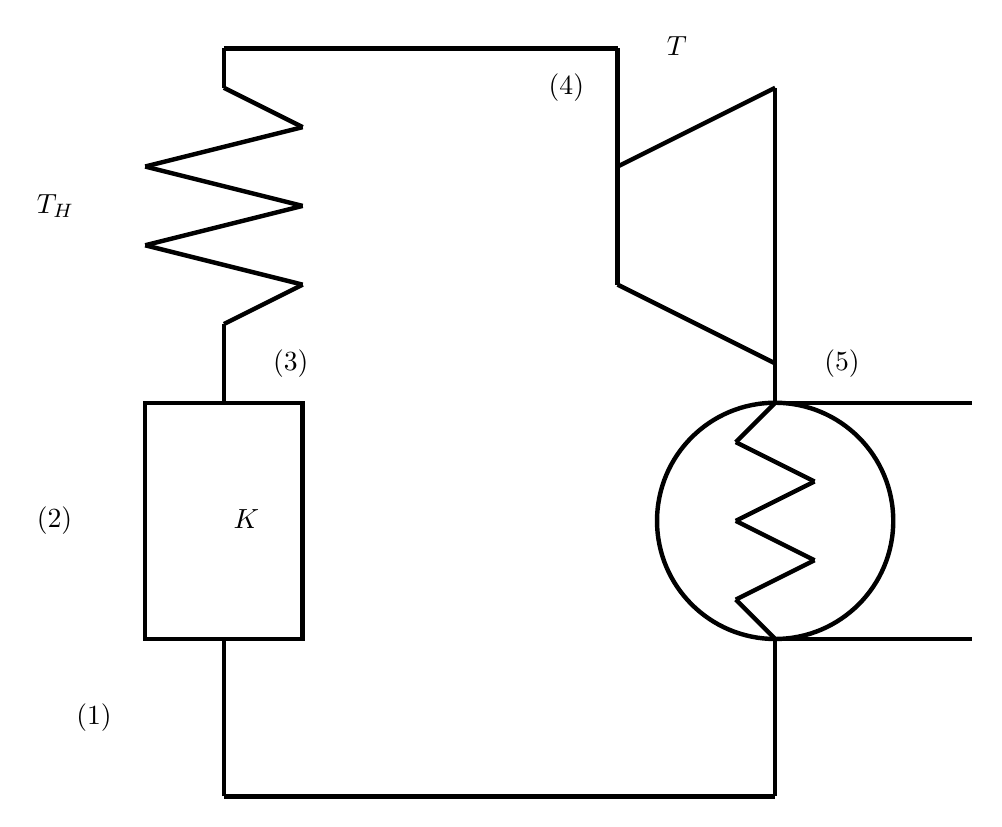
\begin{tikzpicture}
	% Rács és vágómaszk
	%\draw[step=1cm, gray, very thin] (-8, -5) grid (8, 5);
	
	\draw[ultra thick] (-3.5,-5)--(3.5,-5);
	\draw[ultra thick] (3.5,-5)--(3.5,-3);
	\draw[ultra thick] (-3.5,-5)--(-3.5,-3);
	
	%kazán
	\draw[ultra thick] (-4.5, 0) rectangle (-2.5,-3);
	
	%lecsapató 
	\draw[ultra thick] (3.5,-1.5) circle (1.5);
	\draw[ultra thick] (3.5,-3)--(6,-3);
	\draw[ultra thick] (3.5,0)--(6,0);
	
	\draw[ultra thick] (3.5,-3)--(3,-2.5);
	\draw[ultra thick] (3,-2.5)--(4,-2);
	\draw[ultra thick] (4,-2)--(3,-1.5);
	
	\draw[ultra thick] (3,-1.5)--(4,-1);
	\draw[ultra thick] (4,-1)--(3,-0.5);
	
	\draw[ultra thick] (3,-0.5)--(3.5,0);
	
	%turbina
	\draw[ultra thick] (3.5,0)--(3.5,4);
	\draw[ultra thick] (3.5,4)--(1.5,3);
	\draw[ultra thick] (3.5,0.5)--(1.5,1.5);
	\draw[ultra thick] (1.5,3)--(1.5,1.5);
	\draw[ultra thick] (1.5,3)--(1.5,4.5);
	
	%túlhevítő
	\draw[ultra thick] (-3.5,1)--(-3.5,0);
	
	\draw[ultra thick] (-3.5,1)--(-2.5,1.5);
	\draw[ultra thick] (-4.5,2)--(-2.5,1.5);
	
	\draw[ultra thick] (-4.5,2)--(-2.5,2.5);
	\draw[ultra thick] (-4.5,3)--(-2.5,2.5);
	
	\draw[ultra thick] (-4.5,3)--(-2.5,3.5);
	\draw[ultra thick] (-3.5,4)--(-2.5,03.5);
	
	\draw[ultra thick] (-3.5,4)--(-3.5,4.5);
	\draw[ultra thick] (-3.5,4.5)--(1.5,4.5);
	
	%felíratok
		%számok
	\node[anchor=west] at (4, 0.5) {$(5)$};
	\node[anchor=west] at (0.5, 4) {$(4)$};
	\node[anchor=west] at (-3, 0.5) {$(3)$};
	\node[anchor=west] at (-6, -1.5) {$(2)$};
	\node[anchor=west] at (-5.5, -4) {$(1)$};
		%betűk
	\node[anchor=west] at (-6, 2.5) {$T_{H}$};
	\node[anchor=west] at (-3.5, -1.5) {$K_{}$};
	\node[anchor=west] at (2, 4.5) {$T_{}$};
	
	\end{tikzpicture}
	\caption{Körfolyamat ábra}
\end{figure}


%Körfolyamat diagram
\begin{figure}[h]
	\centering
	\label{figure:guh7ud-vgtsd}
	\begin{tikzpicture}
	% Rács és vágómaszk
	%\draw[step=1cm, gray, very thin] (-1.5, -1) grid (14.5, 11);
	%\clip (-1.5, -1) rectangle (14.5, 11);
	
	% A tengelykeresztet az axis környezet hozza létre
	\begin{axis}[
	width=16cm, height=12cm,
	xmin=0, xmax=10.8,
	ymin=0, ymax=475, 
	axis lines = middle,
	axis line style={->},
	xlabel=$s \left(\si{\kilo\joule\per\kilogram\kelvin}\right)$, 
	xlabel style={
		at=(current axis.right of origin), 
		anchor=north east
	}, 
	ylabel=$T \left(\si{\degreeCelsius}\right)$, 
	ylabel style={
		at=(current axis.above origin), 
		anchor=north east
	},
	xtick={1, 2, 3, 4, 5, 6, 7, 8, 9},
	ytick={100, 200, 300, 400}
	]
	
	% Az adat az MHFGY Wolfram-jegyzetfüzetből származik
	
	% A nedves gőzmező fázishatárai
	\addplot[thick] table {./guh7ud/ts.txt};
	
	
	
	\end{axis}
	
	\end{tikzpicture}
	\caption{Víz-gőz $T-s$ diagram}
\end{figure}
\pagebreak

\noindent A feladat célja a termikus hatásfok kiszámítása, amelyet a következő összefüggésekkel tudunk számolni:

\begin{equation*}
\eta_{T}= \dfrac{w_{t}}{q_{be}}
\end{equation*}
\noindent ,valamint:
\begin{equation*}
q_{be}= h_{4}-h_{1}
\end{equation*}
\begin{equation*}
q_{el}= h_{5}-h_{1}
\end{equation*}
\begin{equation*}
w_{t}= q_{be}-q_{el}=h_{4}-h_{5}
\end{equation*}


\noindent A $h_{4}$ értékeink ahogy az ábrán is látható a turbina előtti érték, az-az a feladatleírásban megadott. Azonban a $h_{5}$ értékeket a táblázatból nyert adatokból kell kiszámolnunk. A számolásnál figyelembe kell venni, hogy a táblázati értékeink telítésre vonatkoznak, azonban a $h_{5}$ nem telítési érték. Az tudjuk, hogy a $h'_{}$ értékek az $x_{}=0$ telítési értékhez, a $h''_{}$ pedig az $x_{}=1$ telítési értékhez, valamint azt is tudjuk, hogy e két érték között az entalpia változás arányos az entrópia megváltozással (lásd $T-s$ diagram). Az iméntiek alapján:

\begin{equation*}
h_{5}=\dfrac{h''_{}-h'_{}}{s''_{}-s'{}} \cdot (s_{}-s'_{}) + h'_{}
\end{equation*}
\pagebreak
\noindent Az így kapott megoldások:
\begin{figure}[h]
	\centering
	\label{figure:sm}
	\begin{tikzpicture}
	% Rács és vágómaszk
	%\draw[step=1cm, gray, very thin] (-8, 0) grid (8, 5);
	
	%oszlop1
	\node[anchor=west] at (-4.5, 4) {$p_{k}$ $ \si{\bar}$};
	\node[anchor=west] at (-4.5, 3) {$\Delta s$ $ \si{\kilo\joule\per\kilo\gram\kelvin}$};	
	\node[anchor=west] at (-4.5, 2) {$\Delta h$ $ \si{\kilo\joule\per\kilo\gram}$};
	\node[anchor=west] at (-4.5, 1) {$h_{5} $ $\si{\kilo\joule\per\kilo\gram}$};
	\node[anchor=west] at (-4.5, 0) {$\eta_{T}$ };
	
	
	%oszlop2
	\node[anchor=west] at (-1.5, 4) {$0.5$};
	\node[anchor=west] at (-1.5, 3) {$6.5$};
	\node[anchor=west] at (-1.5, 2) {$2305$};
	\node[anchor=west] at (-1.5, 1) {$2466$};
	\node[anchor=west] at (-1.5, 0) {$24.1\%$};

	
	%oszlop3
	\node[anchor=west] at (1.5, 4) {$0.2$};
	\node[anchor=west] at (1.5, 3) {$7.1$};
	\node[anchor=west] at (1.5, 2) {$2359$};
	\node[anchor=west] at (1.5, 1) {$2343$};
	\node[anchor=west] at (1.5, 0) {$27.5 \%$};

	
	%oszlop4
	\node[anchor=west] at (4.5, 4) {$0.1$};
	\node[anchor=west] at (4.5, 3) {$7.56$};
	\node[anchor=west] at (4.5, 2) {$2396$};
	\node[anchor=west] at (4.5, 1) {$2234$};
	\node[anchor=west] at (4.5, 0) {$30.8\%$};

	
	\end{tikzpicture}
\end{figure}

\subsubsection*{b) Mekkora lesz a körfolyamat irreverzibilis változatának termodinamikai hatásfoka, ha a turbina utáni fajlagos gőztartalom $0.993;$ $0.955,$ ill. $0.94$ ?}
\noindent Irreverzibilis Rankine-Clausius körfolyamatnál a technikai munka csökken, a csökkenés oka, hogy a technikai munka kárára növekszik az entrópia, amely felhasználás szempontjából nem tekinthető hasznos munkának, ezzel csökkentve a hatásfokot. Az előbbiek miatt megnövekedik a $h_{5}^{*}$, amelyet a következő módon számolhatunk:
\begin{equation*}
h_{5}^{*}= \dfrac{\Delta h_{}}{\Delta s_{}} \cdot x_{2} + h'_{}
\end{equation*}
\noindent Az így kapott értékeket behelyettesítve az alábbi egyenletbe kapjuk meg a termodinamikai hatásfokokat:
\begin{equation*}
\eta_{TD}= \dfrac{h_{4}-h_{5}^{*}}{h_{4}-h_{5}}
\end{equation*}
\noindent Az így kapott értékeink rendre:
\begin{equation*}
\eta_{TD-\SI{0.5}{\bar}}= 0.76
\end{equation*}
\begin{equation*}
\eta_{TD-\SI{0.2}{\bar}}= 0.8
\end{equation*}
\begin{equation*}
\eta_{TD-\SI{0.1}{\bar}}= 0.78
\end{equation*}

% Oldaltörés
\pagebreak